%! TEX root = ../thesis.tex
\chapter{Proposed Solution}\label{ch:solution}

The image processing pipeline described in this thesis aims to be suitable for
content based image retrieval using hand-drawn sketches for querying. The main
interest was to evaluate how well the fast discrete curvelet transform (FDCT)
\autocite{candes_fast_2006} is able to represent the lines in hand-drawn
sketches as well as salient edges in photos or paintings. To explore the
effects of preprocessing and signature extraction, several variations of the
pipeline have been implemented. The used preprocessing steps include applying
the sobel operator, extracting a canny edge map or determining segment borders
using the $gPb$ algorithm published in \autocite{arbelaez_contour_2011}.
Signatures are constructed using both, global curvelet features, and a
bag-of-features approach similar to what was described in
\autocite{sivic_video_2003} and \autocite{eitz_sketch-based_2010}.

The following sections will describe the variations of the processing stages
\emph{image acquisition}, \emph{signature extraction}, and \emph{ranking}. To
reference the individual variations unambigiously, labels like LUMA will
be introduced for each component.

\section{Image Acquisition}

% input domains
Since one premise of the system is that hand-drawn sketches are compared with a
large body of images from various sources, a division into two input domains
seems obvious. The first domain, the domain of query sketches, is quite narrow,
because we can characterize its members as binary images with large, smooth
areas separated by discontinuities along curves. The database images, that make
up the second domain, are not subject to such assumptions. They may be color
photographs (Figure \ref{fig:input_example_color}), paintings, computer
renderings or black-and-white sketches.

\paragraph{LUMA}

Because the fast discrete curvelet transform used in every variant of the
signature extraction step takes a single 2D matrix as input, images with more
than one color channel need to be reduced to one channel. The RGB values from
the benchmark dataset have therefore been converted to greyscale images using
the definition of luma according to ITU standards \autocite{_parameter_2002}
(Figure \ref{fig:input_example_luma}).  Each pixel with red, green and blue
values $(R, G, B)$ is mapped to a luminance value $Y$ using
\begin{equation*}
    Y = \frac{299}{1000}R + \frac{587}{1000}G + \frac{114}{1000}B.
\end{equation*}

\paragraph{SOBEL}

In order to make comparing the query sketch to the database images more
effective, an edge extraction algorithm can be applied to each database image.
The Sobel operator calculates horizontal and vertical gradients by convolving
the image with the $3 \times 3$ kernels
\begin{equation*}
    K_x =
    \begin{bmatrix}
        -1 & 0 & 1 \\
        -2 & 0 & 2 \\
        -1 & 0 & 1
    \end{bmatrix}
    \text{ and }
    K_y =
    \begin{bmatrix}
        -1 & -2 & -1 \\
         0 &  0 &  0 \\
         1 &  2 &  1
    \end{bmatrix}
\end{equation*}
to obtain the directional gradients $G_x$ and $G_y$. The overall response is
the gradient magnitude $G$ at each pixel location (Figure
\ref{fig:input_example_sobel}):
\begin{equation*}
    G = \sqrt{G_x^2 + G_y^2}
\end{equation*}

\paragraph{CANNY}

A slightly more complex way to extract edges is the Canny edge detector
\autocite{canny_computational_1986}. Intially, the image is smoothed via a
convolution with a small gaussian kernel to reduce the susceptibility to noise,
even though this increases the localization error of the edge detection. On the
smoothed image the gradient magnitude is calculated using the Sobel operator
described above. The angle of the gradient can be calculated from the
directional gradients $G_x$ and $G_y$ using
\begin{equation*}
    \Theta = \arctan{\frac{G_x}{G_y}}
\end{equation*}
and quantized into bins for $0 \degree$, $45 \degree$, $90 \degree$ and $135
\degree$. Thin edges can be obtained from the gradient magnitudes by performing
non-maximum suppression along the direction perpendicular to the gradient
direction, e.g. a pixel is marked as being on a $90 \degree$ edge if its
magnitude is larger than the magnitudes north and south of its location. To
avoid lines being broken up by noisy fluctiations, the edges are traced along
their direction and gaps are filled in if the signal within the gap is above a
certain threshold. The result is a binary edge map of the whole image (Figure
\ref{fig:input_example_canny}).

\begin{figure}[h]
    \centering
    \subfloat[Original image]{%
        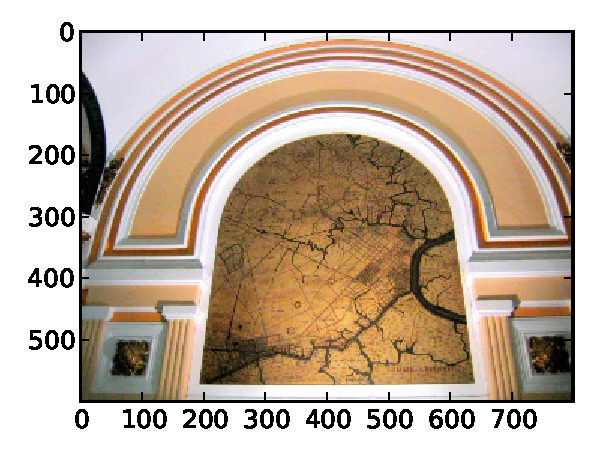
\includegraphics[width=0.45\textwidth]{input_example_color}%
        \label{fig:input_example_color}%
    }
    \quad
    \subfloat[Image after luma conversion]{%
        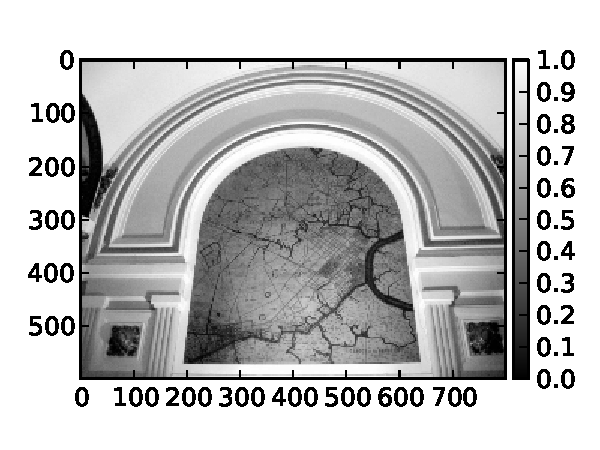
\includegraphics[width=0.45\textwidth]{input_example_luma}%
        \label{fig:input_example_luma}%
    }
    \quad
    \subfloat[Image after Sobel operator]{%
        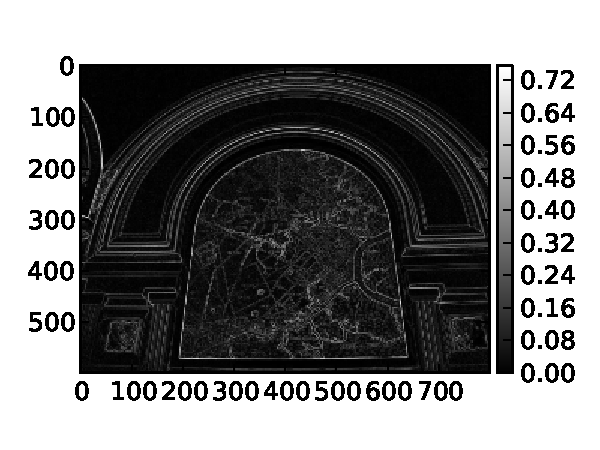
\includegraphics[width=0.45\textwidth]{input_example_sobel}%
        \label{fig:input_example_sobel}%
    }
    \quad
    \subfloat[Image after Canny operator]{%
        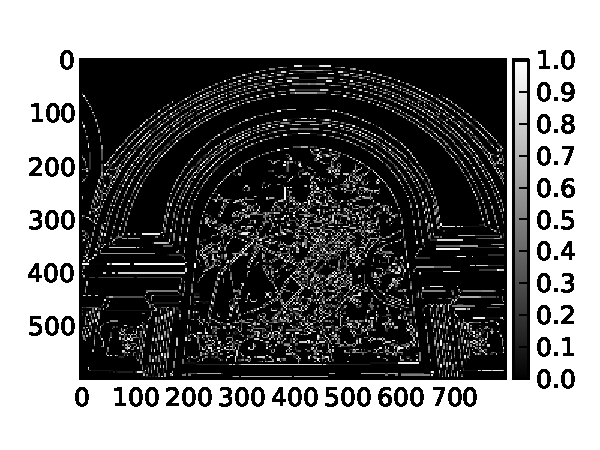
\includegraphics[width=0.45\textwidth]{input_example_canny}%
        \label{fig:input_example_canny}%
    }
    \caption[Image aquisition variants]{
    }
    \label{fig:input_examples}
\end{figure}

\section{Signature Extraction}

Each method of signature extraction described in this section has the fast
discrete curvelet transform at its heart. The curvelet transform has two main
parameters, that influence the result: The number of angles $N_{\theta}$ used
at the coarest scale and the number of scales $N_j$, which corresponds to the
number of concentric squares shown in \ref{fig:curvelet_discrete_tilings}.
Experiments conducted to determine the optimal values of these parameters have
shown that using more scales than 4 does not provide benefits that would
justify the increased amount of processing time. Furthermore, since the
coarsest scale is non-directional, as explained in section
\ref{sec:background_cct}, it is ignored in further computations.

The response image generated by the FDCT for each pair of scale and angle is
too large to be considered for the signature directly. Therefore the response
image $C_{s, \theta}$ for scale $s$ and angle $\theta$ is subdivided into $n^2$
equally sized grid cells $G_{s, \theta, x, y}$ with $x, y \in 1, 2, \dots, n$:
\begin{equation*}
    C_{s,\theta} =
    \begin{bmatrix}
        G_{s,\theta,1,1} & G_{s,\theta,1,2} & \cdots & G_{s,\theta,1,n} \\
        G_{s,\theta,2,1} & G_{s,\theta,2,2} & \cdots & G_{s,\theta,2,n} \\
        \vdots  & \vdots  & \ddots & \vdots  \\
        G_{s,\theta,n,1} & G_{s,\theta,n,2} & \cdots & G_{s,\theta,n,n} \\
    \end{bmatrix}
\end{equation*}
For each of these grid cells, the mean $\bar{C}_{s, \theta}$ is calculated:
\begin{align*}
    \bar{C}_{s,\theta} &=
    \begin{bmatrix}
        mean(G_{s,\theta,1,1}) & mean(G_{s,\theta,1,2}) & \cdots & mean(G_{s,\theta,1,n}) \\
        mean(G_{s,\theta,2,1}) & mean(G_{s,\theta,2,2}) & \cdots & mean(G_{s,\theta,2,n}) \\
        \vdots  & \vdots  & \ddots & \vdots  \\
        mean(G_{s,\theta,n,1}) & mean(G_{s,\theta,n,2}) & \cdots & mean(G_{s,\theta,n,n}) \\
    \end{bmatrix} \\
    &=
    \begin{bmatrix}
        \bar{c}_{s,\theta,1,1} & \bar{c}_{s,\theta,1,2} & \cdots & \bar{c}_{s,\theta,1,n} \\
        \bar{c}_{s,\theta,2,1} & \bar{c}_{s,\theta,2,2} & \cdots & \bar{c}_{s,\theta,2,n} \\
        \vdots  & \vdots  & \ddots & \vdots  \\
        \bar{c}_{s,\theta,n,1} & \bar{c}_{s,\theta,n,2} & \cdots & \bar{c}_{s,\theta,n,n} \\
    \end{bmatrix}
\end{align*}

\subsection{Global Features}

\paragraph{MEAN}

The global approach to signature extraction simply takes the family of matrices
$\bar{C}_{s, \theta}$ and concatenates them as the image signature.

\subsection{Local Features}

The local feature extraction methods used here follow the bag-of-features
approach, that aims to represent an image using a set of local feature
descriptions or "visual words" similar to what was described in
\autocite{sivic_video_2003}. The exact way to extract the words will be
detailed towards the end of this section.

The set of visual words extracted from the images are diverse and hard to
compare. In order to create meaningful image signatures from these words, the
whole set is condensed into a dictionary using k-means clustering. As already
discussed in \ref{sec:anatomy_signature_extraction}, the goal thereof is to
derive a dictionary of predefined size that contains the visual words
corresponding to the most discriminating features of the images in the image
database.

\paragraph{PMEAN}

Continuing from the set of matrices $\bar{C}_{s, \theta}$, this algorithm
densely samples 

\paragraph{PMEAN2}

TBD

\section{Ranking}

TBD

%\section{Input Format}
%\begin{itemize}
    %\item Luma component (Y') of Y'UV representation
    %\item Gradient magnitude of Sobel operator of luma component
    %\item Canny edge map of luma component
    %\item gPb
%\end{itemize}

%\section{Feature Extraction}
%\begin{itemize}
    %\item Global features: mean and standard deviation
    %\item Local features: visual words via k-means clustering
    %\item great comparison of sampling for k-means clustered vws [nowak06]
%\end{itemize}

%\section{Distance Metric}
%\begin{itemize}
    %\item Euclidean Distance
    %\item cosine distance?
    %\item EMD?
%\end{itemize}

%\begin{figure}
    %\scriptsize
    %\begin{tikzpicture}[
            %node distance=1em and 1em,
            %every node/.style={font=\sf},
            %point/.style={},
            %rowHeader/.style={
                %draw=black,
                %text width=5.5em,
            %},
            %colHeader/.style={
                %draw=black,
            %},
            %block/.style={
                %rectangle,
                %draw=black!80, thick,
                %fill=black!10,
                %text width=5.5em,
                %text centered,
                %minimum height=2em,
                %anchor=north,
            %},
            %flow/.style={
                %->,
                %draw=black!40,
                %ultra thick,
            %}
        %]
        %\def\brshift{0em and 2em};

        %% column headers
        %\node[rowHeader] (hCol1) {};
        %\node[rowHeader, right=of hCol1] (hCol2) {};
        %\node[rowHeader, right=of hCol2] (hCol3) {};
        %\node[rowHeader, right=of hCol3] (hCol4) {};
        %\node[rowHeader, right=of hCol4] (hCol5) {};
        %\node[rowHeader, right=of hCol5] (hCol6) {};

        %% row headers
        %\node[colHeader, minimum height=3em, below left=1em and 0em of hCol1] (hRow1) {};
        %\node[colHeader, minimum height=3em, below=of hRow1] (hRow2) {};
        %\node[colHeader, minimum height=3em, below=of hRow2] (hRow3) {};

        %\node[block, minimum height=23em] at (hCol1 |- hRow1.north) (readImage) {Read Image};

        %\node[block] at (hCol2 |- hRow1.north) (extractLuma) {Extract Luma};
        %\node[block] at (hCol2 |- hRow2.north) (applySobel) {Apply Sobel Operator};
        %\node[block] at (hCol2 |- hRow3.north) (applyCanny) {Apply Canny Operator};

        %\node[block, minimum height=11em] at (hCol3 |- hRow1.north) (applyCurvelet) {Apply Curvelet Transform};

        %\node[block, minimum height=11em] at (hCol4 |- hRow1.north) (sample) {Determine Samples};

        %\node[block, minimum height=11em] at (hCol5 |- hRow1.north) (calculateMeans) {Calculate Means};

        %\node[block, minimum height=11em] at (hCol6 |- hRow1.north) (rankEuclidean) {Rank using Euclidean Metric};

        %\foreach \row in {1, 2, 3} {
            %\draw[flow] (hCol1.east |- hRow\row.center) -- (hCol2.west |- hRow\row.center);
            %\draw[flow] (hCol2.east |- hRow\row.center) -- (hCol3.west |- hRow\row.center);
            %\draw[flow] (hCol3.east |- hRow\row.center) -- (hCol4.west |- hRow\row.center);
            %\draw[flow] (hCol4.east |- hRow\row.center) -- (hCol5.west |- hRow\row.center);
            %\draw[flow] (hCol5.east |- hRow\row.center) -- (hCol6.west |- hRow\row.center);
        %}
        %%\def\f1{hRow1.center}
        %%\draw[flow] (\f1 -| readImage.east) -- (\f1 -| extractLuma.west);
        %%\draw[flow] (\f1 -| extractLuma.east) -- (\f1 -| applyCurvelet.west);
        %%\draw[flow] (\f1 -| applyCurvelet.east) -- (\f1 -| sample.west);
        %%\draw[flow] (\f1 -| sample.east) -- (\f1 -| calculateMeans.west);

        %%\def\f2{hRow2.center}
        %%\draw[flow] (\f2 -| readImage.east) -- (\f2 -| applySobel.west);
    %\end{tikzpicture}
%\end{figure}
